% !TeX spellcheck = de_DE
% !TeX encoding = UTF-8
% !TeX root = ../thesis.tex

\chapter{Appendix}

\section{MORE: Equations}\label{more_appendix}
Forming the Lagrangian for the constraint optimization problem we get
\begin{align*} \mathfrak{L}(\pi, \eta, \omega) = 
\int \pi(\theta) \mathcal{R}_{\theta} d\theta \; + \; 
\eta  \left(\epsilon - \int \pi(\theta) \text{ log}
 \frac{\pi(\theta)}{q(\theta)} d\theta\right)
 - \; \omega \left(\beta + \int \pi(\theta) \text{ log}(\pi(\theta)) d\theta\right)
\end{align*}

Optimizing the Lagrangian by computing the derivative with respect
to the mean and covariance matrix yields
\begin{align*}
\pi(\theta) \propto q(\theta)^{\eta/(\eta+\omega)} 
\text{exp}\left(\frac{\mathcal{R}_\theta}{\eta + \omega}\right)
\end{align*}
the solution depends on the quadratic and linear term
of the surrogate model and the
Lagrangian multipliers
$\eta$ and $\omega$. These in turn can be obtained by
minimizing the dual function:
\begin{align}
  \label{eq:dual}
  g(\eta,\omega) = \eta\epsilon - \omega\beta + (\eta - \omega) \text{log}
\left(\int q(\theta)^{\frac{\eta}{\eta + \omega}}
  \text{exp}\left(\frac{\mathcal{R}_\theta}{\eta + \omega}\right) d\theta \right)
\end{align}

Assuming we are given a quadratic surrogate model
$$ \mathcal{R}_\theta \approx \theta^T \mathbf{R} \theta + \theta^T \mathbf{r} + r_0 $$
we can solve the dual function in closed form.
$$ g(\eta, \omega) = \eta \epsilon - \beta \omega
+ \frac{1}{2} \left(\mathbf{f}^T \mathbf{F} \mathbf{f}
  - \eta \mathbf{b}^T \mathbf{Q}^{-1}
  \mathbf{b} - \eta \log |2\pi \mathbf{Q}|p
  + (\eta + \omega) \log |2\pi (\eta + \omega)
\mathbf{F}| \right) $$
with $\mathbf{F} = (\eta \Sigma^{-1} - 2 \mathbf{R})^{-1}$ and
$\mathbf{f} = \eta \Sigma^{-1} \mu + \mathbf{r}$


\section{Gaussian probability function}\label{gauss_pdf}
A random variable $x \in \mathbb{R}^n$ has a Gaussian distribution with mean
$m \in \mathbb{R}^n$ and covariance $P \in \mathbb{R}^{n\times n}$ if its
probability density has the form
$$ \mathcal{N}(x | m, P) = \frac{1}{(2\pi)^{n / 2} |P|^{1/2}}
\text{exp} \left( -\frac{1}{2} (x - m)^T P^{-1} (x-m) \right) $$
where $|P|$ is the determinant of the matrix $P$.

\section{Hyperparameter Search}
\label{appendix:par_search}
Here we first describe the different parameters
that are optimized
then present results and observations from
our hyperparameter search.

\subsubsection{MORE parameters}
\begin{itemize}
\item KL-Bound $\epsilon$
\item entropy-loss bound $\beta$
\end{itemize}
\subsubsection{RLS parameters}
\begin{itemize}
\item model noise $\mathbf{Q}$
\item measurement noise $\sigma^2$
\end{itemize}

\subsubsection{Configurations}
The best configurations we found for our tasks

- table Rosenbrock

- table reaching task

\begin{table}[htp]
  \centering
  \begin{tabular}{lccc} \toprule
    Task (1500 MORE Iterations)
    & Least Squares & RLS with Pool \\ \midrule
    Rosenbrock Function 15D & 16 & 30 \\ \bottomrule
  \end{tabular}
  \caption{
    Computational time for Rosenbrock function.
  }
  \label{tab:table}
\end{table}

\begin{table}[htp]
  \centering
  \begin{tabular}{lccc} \toprule
    Task (300 MORE Iterations)
    & Least Squares & RLS with Pool & RLS without Pool  \\ \midrule
    Via-point Reaching Task & 52 & 102 & 50 \\ \bottomrule
  \end{tabular}
  \caption{
    Computational time for via-point task.
  }
  \label{tab:table}
\end{table}

- configurations of best results list parameters used
for best performing algorithm used in plots

- include extensive hyperparameter search figures and tables

- table for runtimes

\subsection{Further Tests and Observations}
In \Cref{fig:noise_weighting} the influence of adding model noise is
illustrated

 \begin{figure}[ht!]
  \centering
     % This file was created by tikzplotlib v0.9.8.
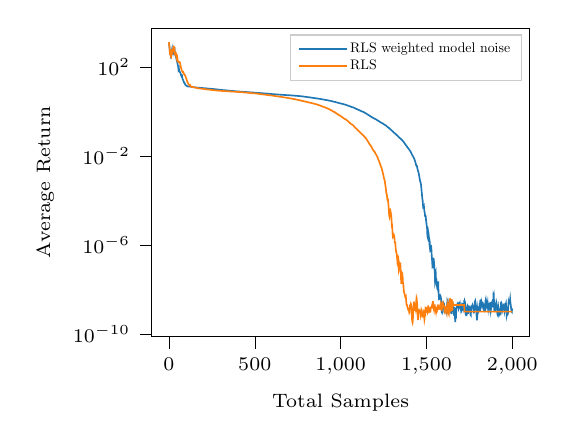
\begin{tikzpicture}

\definecolor{color0}{rgb}{0.12156862745098,0.466666666666667,0.705882352941177}
\definecolor{color1}{rgb}{1,0.498039215686275,0.0549019607843137}

\begin{axis}[
legend cell align={left},
legend style={
  fill opacity=0.8,
  draw opacity=1,
  text opacity=1,
  draw=white!80!black,
  nodes={scale=0.5, transform shape}
},
log basis y={10},
tick align=outside,
ticklabel style = {font=\scriptsize},
xlabel={\scriptsize Total Samples},
ylabel={\scriptsize Average Return},
tick pos=left,
height=5.5cm,
x grid style={white!69.0196078431373!black},
xmin=-99.95, xmax=2098.95,
xtick style={color=black},
y grid style={white!69.0196078431373!black},
ymin=7.67181916900223e-11, ymax=5373.42633809779,
ymode=log,
ytick style={color=black}
]
\addplot [semithick, color0]
table {%
0 1261.58662207
1 1069.84022662
2 908.53463754
3 808.26797976
4 664.2573285
5 544.17778658
6 427.26584709
7 350.17443961
8 436.39236328
9 554.68414779
10 371.38025251
11 305.51130862
12 274.91889012
13 281.86121367
14 337.74637881
15 408.14073112
16 489.03742492
17 529.82654175
18 583.2742166
19 466.13453049
20 440.04423248
21 467.25055719
22 493.98740142
23 543.06282731
24 549.54324913
25 520.210443
26 452.14256463
27 429.45750703
28 460.87567673
29 621.53001738
30 536.91523268
31 599.54638036
32 766.46074554
33 592.26571227
34 475.95301651
35 451.62457084
36 433.18937315
37 393.02532902
38 356.34026053
39 337.67725795
40 303.60116972
41 276.97367039
42 258.07426955
43 244.62537501
44 215.47596287
45 206.10588888
46 190.73243032
47 178.8760273
48 168.99371295
49 155.6198791
50 139.45883765
51 128.00503405
52 115.34974186
53 111.1071458
54 98.97199457
55 84.66210874
56 90.27579487
57 113.69407819
58 82.33389269
59 74.79093733
60 66.63540641
61 62.22191814
62 62.43268869
63 59.50523251
64 58.48334918
65 55.15269319
66 53.5718504
67 51.84415795
68 50.36717416
69 46.30581953
70 43.06356017
71 41.37264984
72 40.6103574
73 38.7631355
74 39.80294583
75 42.13878715
76 41.82092123
77 35.37507266
78 31.95620597
79 28.99961547
80 27.79261626
81 26.75332966
82 26.17769388
83 24.85641588
84 24.17239304
85 23.0150887
86 21.4325936
87 20.4804809
88 19.77590608
89 19.22236911
90 19.50141105
91 19.15450579
92 18.03753713
93 17.39024194
94 16.52563666
95 15.96068063
96 15.48273358
97 15.25968124
98 14.75340543
99 14.45036321
100 14.35891175
101 14.2311318
102 14.0700711
103 14.01643638
104 14.01359013
105 13.7548436
106 13.52615831
107 13.27143822
108 13.16336392
109 13.18996018
110 13.15561772
111 13.19406519
112 13.15239066
113 13.0725682
114 13.12134761
115 13.11769232
116 12.98143396
117 12.94581418
118 12.98791312
119 12.9410632
120 12.90137477
121 12.89803711
122 12.8849145
123 12.91273429
124 12.85258014
125 12.80375893
126 12.74089422
127 12.66948975
128 12.59538756
129 12.54344079
130 12.50759113
131 12.4926344
132 12.45238305
133 12.40712234
134 12.36528883
135 12.33777717
136 12.31223303
137 12.30190935
138 12.26709
139 12.23321037
140 12.19693512
141 12.1632533
142 12.13328379
143 12.09973399
144 12.0710788
145 12.05050076
146 12.02602066
147 12.00407294
148 11.98377698
149 11.9635154
150 11.94293372
151 11.92533463
152 11.90701694
153 11.88679121
154 11.86117134
155 11.83287132
156 11.80633862
157 11.7812156
158 11.75990129
159 11.73190943
160 11.70461602
161 11.68175273
162 11.66239007
163 11.64542962
164 11.62794118
165 11.61381089
166 11.59827664
167 11.59239904
168 11.56838119
169 11.54786218
170 11.52683444
171 11.50771362
172 11.4923727
173 11.47583484
174 11.4593699
175 11.4442614
176 11.4347612
177 11.41927966
178 11.39920138
179 11.37846358
180 11.35791033
181 11.33840118
182 11.3238626
183 11.31082657
184 11.29370794
185 11.27397854
186 11.25722137
187 11.23874738
188 11.22109832
189 11.20503729
190 11.19295461
191 11.18342844
192 11.1670387
193 11.14763108
194 11.1286088
195 11.11044027
196 11.09075442
197 11.07168228
198 11.05853016
199 11.03862917
200 11.01888598
201 11.0064185
202 10.99761597
203 10.98507235
204 10.96512538
205 10.94613107
206 10.92942544
207 10.92065091
208 10.91236276
209 10.89885015
210 10.88358001
211 10.8650237
212 10.84183792
213 10.82127928
214 10.80265975
215 10.78607993
216 10.76799738
217 10.75093324
218 10.73185572
219 10.71274612
220 10.69200259
221 10.67225042
222 10.65477973
223 10.6395882
224 10.6279394
225 10.61652599
226 10.60260898
227 10.57621615
228 10.5523792
229 10.53083156
230 10.51178129
231 10.49417341
232 10.47831238
233 10.46175199
234 10.44847792
235 10.43618157
236 10.42433243
237 10.41723427
238 10.41098888
239 10.39385645
240 10.37954568
241 10.35713783
242 10.331044
243 10.30538682
244 10.28208397
245 10.2589482
246 10.23693589
247 10.21490127
248 10.1949087
249 10.17793864
250 10.15937031
251 10.13941289
252 10.11788365
253 10.09865344
254 10.08494583
255 10.0698001
256 10.06131107
257 10.06022954
258 10.05062256
259 10.03066507
260 10.00682796
261 9.99372076
262 9.97210252
263 9.94944255
264 9.92526495
265 9.90336594
266 9.88114127
267 9.85971885
268 9.83935912
269 9.82145292
270 9.80987272
271 9.80062193
272 9.7850496
273 9.76945649
274 9.75716619
275 9.73877824
276 9.73177811
277 9.71707925
278 9.69717083
279 9.67712112
280 9.65109608
281 9.62589223
282 9.60147904
283 9.57704856
284 9.55460504
285 9.53701088
286 9.52005948
287 9.50327244
288 9.48686216
289 9.46916248
290 9.4463004
291 9.42274569
292 9.39986403
293 9.37956105
294 9.35966032
295 9.34420229
296 9.33278071
297 9.32734501
298 9.32038746
299 9.29435895
300 9.26889063
301 9.24483535
302 9.22523608
303 9.20724265
304 9.19231816
305 9.18009188
306 9.16649001
307 9.15149773
308 9.1307198
309 9.1096432
310 9.09003922
311 9.06581581
312 9.04378949
313 9.02340572
314 9.00726038
315 8.99330913
316 8.98357549
317 8.96691508
318 8.95128935
319 8.9393378
320 8.93478682
321 8.95172328
322 8.92367529
323 8.90180491
324 8.88628314
325 8.86924701
326 8.85295883
327 8.84002839
328 8.82855065
329 8.81135548
330 8.79724495
331 8.78875958
332 8.77774278
333 8.76126222
334 8.74730978
335 8.73042783
336 8.71309648
337 8.69801056
338 8.68048007
339 8.66073298
340 8.6422863
341 8.62347322
342 8.60636735
343 8.59090545
344 8.57723824
345 8.56304161
346 8.5514019
347 8.54111382
348 8.52695077
349 8.51220387
350 8.49836824
351 8.48580472
352 8.47223377
353 8.45632858
354 8.4407874
355 8.42613975
356 8.41032056
357 8.39466268
358 8.37802391
359 8.36285836
360 8.3491968
361 8.33489835
362 8.32140666
363 8.30992676
364 8.29947472
365 8.29102597
366 8.2804014
367 8.26549115
368 8.25144877
369 8.24161486
370 8.22844562
371 8.21447694
372 8.20613981
373 8.18831312
374 8.17183876
375 8.1590908
376 8.14881486
377 8.13577193
378 8.12486024
379 8.11579983
380 8.10295801
381 8.09080225
382 8.0774574
383 8.06278661
384 8.04909783
385 8.03545268
386 8.02007344
387 8.00632301
388 7.99151405
389 7.97731771
390 7.96202882
391 7.94755284
392 7.93507059
393 7.92460026
394 7.91324088
395 7.90261519
396 7.89079605
397 7.88040815
398 7.87241694
399 7.86044479
400 7.84695533
401 7.83731444
402 7.8254997
403 7.81442486
404 7.80467752
405 7.79154298
406 7.77944901
407 7.76691091
408 7.75659882
409 7.74468384
410 7.73762131
411 7.73352248
412 7.72002029
413 7.70715959
414 7.69849254
415 7.68871208
416 7.67868683
417 7.66694968
418 7.65603072
419 7.64358839
420 7.63505503
421 7.62362054
422 7.61383629
423 7.60581655
424 7.59587302
425 7.58421981
426 7.57071085
427 7.55948905
428 7.54772261
429 7.53714068
430 7.52794683
431 7.5190668
432 7.51142019
433 7.50641377
434 7.49954824
435 7.49412537
436 7.49097737
437 7.48834488
438 7.47852211
439 7.46892573
440 7.46290018
441 7.45833312
442 7.45501611
443 7.44051544
444 7.42555221
445 7.41166991
446 7.40035869
447 7.39011421
448 7.37962866
449 7.36956216
450 7.35863596
451 7.35022763
452 7.34194618
453 7.33141348
454 7.32043061
455 7.309901
456 7.30036724
457 7.29136581
458 7.28344037
459 7.2761931
460 7.2669954
461 7.25696695
462 7.24663139
463 7.23553285
464 7.22679198
465 7.22005161
466 7.21286135
467 7.20286972
468 7.19354206
469 7.18417236
470 7.17330187
471 7.16160278
472 7.15060842
473 7.1413882
474 7.13355414
475 7.12745467
476 7.12132739
477 7.11685646
478 7.11010153
479 7.10211047
480 7.09197999
481 7.07909622
482 7.06982273
483 7.06145442
484 7.04880246
485 7.03708822
486 7.02733668
487 7.01890904
488 7.01105374
489 7.00496939
490 7.00074854
491 6.99484001
492 6.98540359
493 6.97595119
494 6.96724014
495 6.95899572
496 6.95061616
497 6.94093119
498 6.93145805
499 6.92214688
500 6.91304377
501 6.90288592
502 6.89316934
503 6.88235973
504 6.87223694
505 6.86188371
506 6.85044247
507 6.83992555
508 6.82798376
509 6.81653129
510 6.80610035
511 6.79644528
512 6.7866718
513 6.77655485
514 6.76685609
515 6.75762201
516 6.74794677
517 6.73875166
518 6.73056747
519 6.72546671
520 6.71612908
521 6.70630692
522 6.69588567
523 6.68607387
524 6.67681927
525 6.66845853
526 6.65864894
527 6.64742956
528 6.63703793
529 6.62530726
530 6.61306594
531 6.6017108
532 6.59222789
533 6.58211417
534 6.57418169
535 6.56518643
536 6.55577797
537 6.54701269
538 6.53631452
539 6.52594865
540 6.51552082
541 6.5051114
542 6.49541773
543 6.48496737
544 6.47619958
545 6.46890904
546 6.46252251
547 6.4550054
548 6.44694358
549 6.43992557
550 6.43411424
551 6.42296305
552 6.41149439
553 6.40069789
554 6.38881977
555 6.37923236
556 6.37114981
557 6.36414239
558 6.35452121
559 6.34276642
560 6.33348238
561 6.32717942
562 6.32038812
563 6.31098737
564 6.30349112
565 6.29530826
566 6.28332609
567 6.27061742
568 6.25890447
569 6.24776366
570 6.23650249
571 6.22461053
572 6.21432719
573 6.20762678
574 6.19678581
575 6.18443669
576 6.17292969
577 6.16238334
578 6.15334966
579 6.14743667
580 6.14718725
581 6.14277421
582 6.1380157
583 6.12656336
584 6.11533036
585 6.10827651
586 6.10278166
587 6.10161386
588 6.09295332
589 6.0838854
590 6.0731475
591 6.06130214
592 6.04990654
593 6.04089616
594 6.03248796
595 6.02205136
596 6.01388421
597 6.00373991
598 5.99441898
599 5.9849321
600 5.9758178
601 5.9668067
602 5.95788207
603 5.9508591
604 5.94333027
605 5.93920462
606 5.93472113
607 5.9256079
608 5.91597962
609 5.90398562
610 5.8915462
611 5.88153402
612 5.87373316
613 5.87044707
614 5.8647582
615 5.85472092
616 5.84610281
617 5.83816237
618 5.83114413
619 5.82435643
620 5.81580714
621 5.80723812
622 5.80235605
623 5.79458184
624 5.78696585
625 5.77996322
626 5.77214751
627 5.76473801
628 5.75760236
629 5.75015001
630 5.745883
631 5.73795714
632 5.72984232
633 5.72143487
634 5.7124321
635 5.70341288
636 5.69451824
637 5.68573056
638 5.6822245
639 5.67893903
640 5.66748598
641 5.65448219
642 5.6441674
643 5.63464159
644 5.62606829
645 5.61875305
646 5.6105779
647 5.60378817
648 5.59722932
649 5.5886829
650 5.58092194
651 5.57319989
652 5.56669361
653 5.55836006
654 5.5502663
655 5.5428986
656 5.53652454
657 5.53126573
658 5.52700127
659 5.52253039
660 5.51827337
661 5.51280891
662 5.5069643
663 5.50324215
664 5.49823019
665 5.4929483
666 5.48737707
667 5.48132391
668 5.47382203
669 5.46659964
670 5.45951235
671 5.4514292
672 5.44520232
673 5.44039452
674 5.43244363
675 5.42474824
676 5.41655423
677 5.41025654
678 5.40385188
679 5.39819494
680 5.39340956
681 5.38664892
682 5.37866669
683 5.37141945
684 5.3640959
685 5.35703739
686 5.35026026
687 5.34352878
688 5.33738215
689 5.33206416
690 5.32833312
691 5.32493223
692 5.3201948
693 5.31370777
694 5.30755263
695 5.30085158
696 5.29505596
697 5.28860012
698 5.28255959
699 5.27664787
700 5.27014131
701 5.26466982
702 5.26048231
703 5.25809476
704 5.25336544
705 5.24463727
706 5.23747562
707 5.230579
708 5.2228356
709 5.21546514
710 5.20801414
711 5.20157911
712 5.19517648
713 5.18999016
714 5.18466933
715 5.17857154
716 5.17442173
717 5.16690893
718 5.15934015
719 5.15215305
720 5.14513382
721 5.13895524
722 5.13171848
723 5.12314923
724 5.11474555
725 5.10711731
726 5.10072875
727 5.09549183
728 5.08772923
729 5.07798165
730 5.06933326
731 5.06278675
732 5.05592627
733 5.04715806
734 5.03990698
735 5.03449729
736 5.02649724
737 5.01896527
738 5.0115079
739 5.00420474
740 4.99800725
741 4.99108401
742 4.98626341
743 4.97943738
744 4.97274148
745 4.96485427
746 4.95768794
747 4.95134113
748 4.94455559
749 4.9362477
750 4.92747639
751 4.92111349
752 4.9120115
753 4.90487754
754 4.89444436
755 4.88428752
756 4.87305968
757 4.86414439
758 4.85795306
759 4.85363254
760 4.84680764
761 4.83712898
762 4.82572537
763 4.81658433
764 4.80831238
765 4.80144725
766 4.79544517
767 4.79105893
768 4.78445681
769 4.77832883
770 4.76562186
771 4.75576457
772 4.74534712
773 4.73329531
774 4.72182666
775 4.7113997
776 4.7016571
777 4.69417443
778 4.6857338
779 4.67645073
780 4.66651393
781 4.65615531
782 4.64382297
783 4.63130781
784 4.61842102
785 4.60674457
786 4.59655208
787 4.58562365
788 4.57206901
789 4.56079835
790 4.55063446
791 4.53877557
792 4.52825016
793 4.51536079
794 4.50314999
795 4.4923352
796 4.48297178
797 4.47671101
798 4.46843686
799 4.45843743
800 4.44972491
801 4.43788452
802 4.42870392
803 4.41542992
804 4.40165161
805 4.38891528
806 4.37637858
807 4.36311751
808 4.35170392
809 4.34060324
810 4.32729594
811 4.31634102
812 4.30651981
813 4.29608943
814 4.28861058
815 4.28647116
816 4.28255656
817 4.27967594
818 4.26251775
819 4.24558703
820 4.23074994
821 4.21843361
822 4.21045086
823 4.20751669
824 4.21030066
825 4.19995486
826 4.18306319
827 4.16559296
828 4.14884111
829 4.13430458
830 4.12177845
831 4.11327152
832 4.0992637
833 4.08509551
834 4.07332794
835 4.06061881
836 4.04865202
837 4.0379294
838 4.02771325
839 4.01976927
840 4.01482054
841 4.00591158
842 3.99693063
843 3.98665446
844 3.97789411
845 3.96747706
846 3.95608401
847 3.94477995
848 3.93234895
849 3.92486591
850 3.91634018
851 3.90924411
852 3.8954646
853 3.88257086
854 3.87082142
855 3.85989961
856 3.85292928
857 3.84521289
858 3.83852184
859 3.82617825
860 3.8139301
861 3.80453275
862 3.79460289
863 3.78717744
864 3.78224964
865 3.76774425
866 3.75510377
867 3.7430607
868 3.73288101
869 3.72085158
870 3.70920165
871 3.69920642
872 3.69093651
873 3.67778678
874 3.66547591
875 3.65295546
876 3.64177217
877 3.63105974
878 3.62230078
879 3.61226601
880 3.60161958
881 3.59006255
882 3.57806546
883 3.56715181
884 3.5567296
885 3.54758989
886 3.53804284
887 3.5273217
888 3.51760307
889 3.50674001
890 3.4935806
891 3.48097649
892 3.46970165
893 3.45720173
894 3.44599857
895 3.43598961
896 3.42787677
897 3.41526717
898 3.40306037
899 3.39054859
900 3.37873667
901 3.36882446
902 3.36002567
903 3.35348922
904 3.34860303
905 3.34396692
906 3.33310083
907 3.32508597
908 3.30557277
909 3.28881766
910 3.27645908
911 3.26431539
912 3.25516714
913 3.24722133
914 3.23946713
915 3.22974424
916 3.22511002
917 3.21531352
918 3.20292627
919 3.19051843
920 3.17891696
921 3.16834543
922 3.15859347
923 3.15286162
924 3.15492826
925 3.14409429
926 3.12291018
927 3.1078848
928 3.09451402
929 3.08268833
930 3.07186772
931 3.06077624
932 3.04947465
933 3.03902825
934 3.02953767
935 3.02220733
936 3.01094821
937 2.99668156
938 2.9822773
939 2.96805858
940 2.95609185
941 2.94374445
942 2.93547407
943 2.92536485
944 2.91557238
945 2.90691724
946 2.8976753
947 2.88810731
948 2.87763481
949 2.86392916
950 2.85120207
951 2.83967414
952 2.82455437
953 2.81004832
954 2.79656326
955 2.78177921
956 2.7713204
957 2.75406961
958 2.73767054
959 2.72101451
960 2.70564129
961 2.69275077
962 2.68171888
963 2.67270588
964 2.66486475
965 2.66471768
966 2.65501184
967 2.64335005
968 2.63395915
969 2.62363924
970 2.62318448
971 2.61308166
972 2.59696953
973 2.57357566
974 2.5553233
975 2.54119843
976 2.52739268
977 2.51443928
978 2.5021077
979 2.48932713
980 2.4774632
981 2.46516526
982 2.45566875
983 2.4568777
984 2.43831917
985 2.42230531
986 2.4073878
987 2.3962216
988 2.38507172
989 2.37600004
990 2.3635887
991 2.35220356
992 2.34140683
993 2.33189951
994 2.32242851
995 2.31422819
996 2.30778825
997 2.29783856
998 2.28573312
999 2.27425239
1000 2.26205666
1001 2.25162696
1002 2.24084536
1003 2.23053603
1004 2.22094441
1005 2.21259016
1006 2.20584822
1007 2.20382554
1008 2.20316724
1009 2.19193288
1010 2.18019033
1011 2.16639574
1012 2.1539601
1013 2.14363667
1014 2.13275423
1015 2.12289119
1016 2.1094238
1017 2.0987812
1018 2.08504015
1019 2.07110708
1020 2.05806308
1021 2.04588406
1022 2.03540382
1023 2.02717681
1024 2.02117273
1025 2.01076173
1026 2.00168292
1027 1.99656248
1028 1.99094359
1029 1.98894143
1030 1.98600013
1031 1.96647858
1032 1.94826538
1033 1.93280585
1034 1.91794429
1035 1.90419949
1036 1.89021454
1037 1.87534289
1038 1.86147652
1039 1.84882456
1040 1.83965988
1041 1.82720388
1042 1.81763319
1043 1.80787901
1044 1.79434911
1045 1.78236853
1046 1.77022869
1047 1.75905877
1048 1.7478771
1049 1.73682275
1050 1.72593962
1051 1.71461084
1052 1.70541517
1053 1.69633306
1054 1.69183646
1055 1.68077917
1056 1.67124662
1057 1.65860015
1058 1.65029769
1059 1.63787151
1060 1.62286431
1061 1.60707435
1062 1.59277222
1063 1.57842763
1064 1.56695046
1065 1.55712353
1066 1.54966145
1067 1.54084829
1068 1.53761066
1069 1.5374406
1070 1.52771239
1071 1.51857661
1072 1.50945901
1073 1.5037741
1074 1.49492214
1075 1.48285183
1076 1.47046544
1077 1.45655832
1078 1.44182126
1079 1.42812065
1080 1.41524554
1081 1.40362007
1082 1.39136809
1083 1.38002516
1084 1.36876278
1085 1.35676335
1086 1.3461287
1087 1.33568456
1088 1.32305383
1089 1.31125235
1090 1.30056296
1091 1.29134287
1092 1.28095855
1093 1.27331705
1094 1.26434912
1095 1.25415152
1096 1.24392249
1097 1.23570069
1098 1.22862327
1099 1.21955913
1100 1.20834446
1101 1.19966182
1102 1.18967425
1103 1.18114787
1104 1.17006451
1105 1.16044327
1106 1.1500233
1107 1.14096478
1108 1.13195874
1109 1.12565193
1110 1.11621256
1111 1.10865527
1112 1.09950783
1113 1.0914858
1114 1.08012435
1115 1.07024485
1116 1.06155383
1117 1.05238482
1118 1.04497527
1119 1.03531324
1120 1.02655734
1121 1.02090267
1122 1.01360265
1123 1.00497666
1124 0.99657194
1125 0.98834099
1126 0.97984863
1127 0.97233699
1128 0.96502492
1129 0.95858345
1130 0.95043699
1131 0.94437898
1132 0.93920787
1133 0.93468571
1134 0.92947268
1135 0.92392698
1136 0.91663502
1137 0.90633111
1138 0.89319082
1139 0.88137116
1140 0.87048191
1141 0.86016327
1142 0.85052109
1143 0.84212496
1144 0.83330113
1145 0.82516928
1146 0.81837867
1147 0.81134493
1148 0.80088141
1149 0.7910573
1150 0.78318596
1151 0.77626598
1152 0.76803622
1153 0.75949378
1154 0.75015604
1155 0.74217191
1156 0.73341035
1157 0.7242714
1158 0.71727711
1159 0.70886637
1160 0.70214699
1161 0.69387033
1162 0.68605724
1163 0.67859476
1164 0.67183194
1165 0.66446854
1166 0.65679756
1167 0.64747686
1168 0.63875267
1169 0.63275954
1170 0.62558351
1171 0.61934177
1172 0.61629397
1173 0.61055288
1174 0.6027198
1175 0.59341751
1176 0.58648929
1177 0.58179906
1178 0.57485274
1179 0.56796518
1180 0.55948865
1181 0.5519887
1182 0.54606022
1183 0.54065392
1184 0.53718572
1185 0.53348419
1186 0.52768299
1187 0.52022607
1188 0.51313667
1189 0.50695845
1190 0.50110548
1191 0.49584147
1192 0.49151529
1193 0.48679002
1194 0.48281909
1195 0.47956005
1196 0.4755646
1197 0.47082503
1198 0.46745135
1199 0.46575705
1200 0.45965622
1201 0.45461079
1202 0.45099703
1203 0.44663988
1204 0.44276059
1205 0.43691682
1206 0.4335213
1207 0.43335466
1208 0.42898041
1209 0.42343854
1210 0.41746136
1211 0.41194713
1212 0.40674391
1213 0.40222989
1214 0.39825967
1215 0.39381397
1216 0.38917449
1217 0.38366885
1218 0.37815423
1219 0.37360191
1220 0.36964733
1221 0.36651864
1222 0.36343088
1223 0.35969469
1224 0.35776331
1225 0.35328632
1226 0.34931356
1227 0.34603009
1228 0.3415262
1229 0.33621445
1230 0.33120606
1231 0.32669003
1232 0.32303812
1233 0.31975743
1234 0.31720407
1235 0.31430837
1236 0.31116026
1237 0.30808522
1238 0.3055255
1239 0.30349189
1240 0.30111725
1241 0.29878744
1242 0.29520731
1243 0.2913837
1244 0.28807281
1245 0.28513074
1246 0.28217434
1247 0.28135302
1248 0.27629698
1249 0.27197515
1250 0.2683364
1251 0.26531479
1252 0.26329587
1253 0.25980784
1254 0.25682761
1255 0.25379486
1256 0.25082601
1257 0.24854779
1258 0.24593241
1259 0.24322061
1260 0.24091931
1261 0.23810319
1262 0.23590738
1263 0.23419624
1264 0.23119422
1265 0.22774907
1266 0.22386223
1267 0.22017436
1268 0.21670644
1269 0.21316709
1270 0.20956635
1271 0.20634877
1272 0.20310925
1273 0.20000849
1274 0.19733759
1275 0.19497406
1276 0.19288119
1277 0.19131445
1278 0.18856598
1279 0.1854939
1280 0.18254683
1281 0.17913514
1282 0.17580691
1283 0.1730164
1284 0.17074537
1285 0.16937554
1286 0.16862762
1287 0.16517469
1288 0.16065099
1289 0.15726708
1290 0.15483785
1291 0.15281316
1292 0.15127488
1293 0.15051406
1294 0.14770885
1295 0.14470803
1296 0.14220655
1297 0.13961448
1298 0.13734509
1299 0.1350895
1300 0.13311017
1301 0.13117632
1302 0.12902053
1303 0.12685528
1304 0.12501248
1305 0.12285738
1306 0.1207733
1307 0.11842584
1308 0.11610585
1309 0.11363432
1310 0.11127212
1311 0.1091609
1312 0.10732413
1313 0.10613059
1314 0.10490288
1315 0.10388842
1316 0.10284876
1317 0.10150981
1318 0.10029361
1319 0.09825426
1320 0.09642561
1321 0.09468195
1322 0.09278742
1323 0.09118454
1324 0.0895331
1325 0.08831228
1326 0.08674762
1327 0.08544549
1328 0.08436778
1329 0.08314985
1330 0.08204529
1331 0.08080138
1332 0.07962315
1333 0.07810749
1334 0.07649033
1335 0.07487913
1336 0.07342047
1337 0.07196507
1338 0.07048589
1339 0.06908132
1340 0.06766323
1341 0.06645896
1342 0.06551469
1343 0.06464401
1344 0.06383006
1345 0.06270956
1346 0.0617747
1347 0.06095586
1348 0.06051745
1349 0.05980784
1350 0.05853434
1351 0.05764426
1352 0.05620756
1353 0.05524955
1354 0.05446978
1355 0.05401035
1356 0.05297509
1357 0.05199074
1358 0.05077374
1359 0.04962775
1360 0.04854336
1361 0.04772404
1362 0.04686041
1363 0.04595209
1364 0.0452947
1365 0.04449387
1366 0.04359605
1367 0.04265984
1368 0.04159722
1369 0.04051232
1370 0.03947363
1371 0.03840113
1372 0.03745439
1373 0.03644567
1374 0.03544021
1375 0.03440003
1376 0.03353719
1377 0.03287061
1378 0.0319423
1379 0.03100977
1380 0.03021058
1381 0.02982733
1382 0.02921715
1383 0.02832388
1384 0.02777669
1385 0.02708522
1386 0.02641009
1387 0.02608553
1388 0.02493955
1389 0.02399354
1390 0.02355374
1391 0.02327384
1392 0.02299195
1393 0.02241573
1394 0.02176384
1395 0.02111068
1396 0.02068409
1397 0.02022091
1398 0.02002137
1399 0.01955425
1400 0.01893701
1401 0.01833829
1402 0.01798605
1403 0.01747427
1404 0.01703796
1405 0.01664338
1406 0.01627643
1407 0.01577618
1408 0.01518458
1409 0.01465576
1410 0.01422033
1411 0.01362876
1412 0.01306584
1413 0.01254428
1414 0.01207397
1415 0.01173454
1416 0.01132905
1417 0.01093204
1418 0.010669
1419 0.0103174
1420 0.01002907
1421 0.00971958
1422 0.00958348
1423 0.00920277
1424 0.0088507
1425 0.00858812
1426 0.00832644
1427 0.00801454
1428 0.00767742
1429 0.00733592
1430 0.0069863
1431 0.00661532
1432 0.00630293
1433 0.00597556
1434 0.00567895
1435 0.00541859
1436 0.00502742
1437 0.00468097
1438 0.0043308
1439 0.00402778
1440 0.00378185
1441 0.00359725
1442 0.00351132
1443 0.00357285
1444 0.00351804
1445 0.00349751
1446 0.00309208
1447 0.00275036
1448 0.00250676
1449 0.00233415
1450 0.00223887
1451 0.00214021
1452 0.00202337
1453 0.00187779
1454 0.00173582
1455 0.00157107
1456 0.00146323
1457 0.00133686
1458 0.001232
1459 0.00108678
1460 0.0009735
1461 0.0008795
1462 0.00081166
1463 0.0007374
1464 0.00067798
1465 0.00065624
1466 0.00063967
1467 0.00057404
1468 0.00051385
1469 0.00044665
1470 0.00036451
1471 0.00029328
1472 0.00024231
1473 0.00021216
1474 0.00017599
1475 0.00014064
1476 0.00012008
1477 0.00010531
1478 9.69268676e-05
1479 7.38383378e-05
1480 5.80258686e-05
1481 4.83208994e-05
1482 4.88477882e-05
1483 5.17961104e-05
1484 5.37625116e-05
1485 5.58495523e-05
1486 4.60813455e-05
1487 3.88950983e-05
1488 3.30775833e-05
1489 2.98686661e-05
1490 2.73630851e-05
1491 2.29195074e-05
1492 1.9371692e-05
1493 1.91786727e-05
1494 2.04467208e-05
1495 2.02956073e-05
1496 1.88406704e-05
1497 1.36912449e-05
1498 1.16897394e-05
1499 1.05298489e-05
1500 9.14085419e-06
1501 7.73682759e-06
1502 7.01570909e-06
1503 6.08927862e-06
1504 4.55033626e-06
1505 2.99296641e-06
1506 2.42076439e-06
1507 2.26613637e-06
1508 2.75059718e-06
1509 3.47500154e-06
1510 3.99353958e-06
1511 3.60218448e-06
1512 3.45478539e-06
1513 2.66052922e-06
1514 2.2718646e-06
1515 2.02660285e-06
1516 1.62307054e-06
1517 1.27475544e-06
1518 9.95715641e-07
1519 8.67035524e-07
1520 9.48230986e-07
1521 7.14154961e-07
1522 5.71459018e-07
1523 5.85455492e-07
1524 6.40518544e-07
1525 6.84946154e-07
1526 9.34939733e-07
1527 9.22855292e-07
1528 7.29049639e-07
1529 5.98920531e-07
1530 3.93130925e-07
1531 2.97291944e-07
1532 2.32926875e-07
1533 1.89136764e-07
1534 1.35841803e-07
1535 9.80783193e-08
1536 9.84881819e-08
1537 1.40195163e-07
1538 1.57741339e-07
1539 2.47786669e-07
1540 2.48281903e-07
1541 2.11149785e-07
1542 2.03031964e-07
1543 2.06502707e-07
1544 1.42281027e-07
1545 1.24469366e-07
1546 8.24215274e-08
1547 7.51393516e-08
1548 8.55010399e-08
1549 3.57369924e-08
1550 2.14138917e-08
1551 2.31023602e-08
1552 4.54106553e-08
1553 4.48055598e-08
1554 4.91748163e-08
1555 3.07992598e-08
1556 2.04677085e-08
1557 2.06594138e-08
1558 1.91823917e-08
1559 2.05227803e-08
1560 1.57721785e-08
1561 1.4170078e-08
1562 1.49555751e-08
1563 1.20907111e-08
1564 1.14179782e-08
1565 1.27955731e-08
1566 1.63268744e-08
1567 2.01443417e-08
1568 2.35431285e-08
1569 1.33357459e-08
1570 7.58297837e-09
1571 6.28653039e-09
1572 4.49450515e-09
1573 3.74195541e-09
1574 3.78179266e-09
1575 4.4775754e-09
1576 5.31713486e-09
1577 5.30200244e-09
1578 5.34968163e-09
1579 5.30539538e-09
1580 5.49758585e-09
1581 5.28662692e-09
1582 4.62265318e-09
1583 4.58718593e-09
1584 3.60829026e-09
1585 4.19771551e-09
1586 3.11539094e-09
1587 2.14173967e-09
1588 1.33942225e-09
1589 9.94929727e-10
1590 9.60084637e-10
1591 1.11592315e-09
1592 1.08969877e-09
1593 1.37005663e-09
1594 1.53623558e-09
1595 1.74511322e-09
1596 1.96516667e-09
1597 1.85551909e-09
1598 1.98545963e-09
1599 2.22608344e-09
1600 2.0915281e-09
1601 2.41018326e-09
1602 2.34749911e-09
1603 1.81010264e-09
1604 1.48803436e-09
1605 1.00444166e-09
1606 8.598883e-10
1607 1.14133059e-09
1608 1.50117074e-09
1609 1.27786361e-09
1610 1.30127864e-09
1611 1.22625124e-09
1612 1.22138635e-09
1613 1.46570248e-09
1614 1.57827209e-09
1615 1.63672059e-09
1616 1.44969062e-09
1617 1.25190252e-09
1618 1.45773546e-09
1619 1.25478739e-09
1620 1.71440834e-09
1621 2.47828256e-09
1622 2.28971029e-09
1623 2.17608838e-09
1624 2.3797043e-09
1625 2.63533123e-09
1626 2.30722474e-09
1627 1.52624923e-09
1628 1.22696403e-09
1629 8.17175738e-10
1630 9.43063728e-10
1631 1.22777736e-09
1632 1.65997823e-09
1633 1.71273908e-09
1634 1.65843934e-09
1635 1.72199871e-09
1636 2.17717876e-09
1637 2.32928823e-09
1638 2.4126737e-09
1639 2.02690554e-09
1640 1.92954523e-09
1641 1.55213305e-09
1642 1.12719536e-09
1643 9.33443288e-10
1644 9.03257358e-10
1645 8.97971436e-10
1646 7.95249922e-10
1647 1.14131354e-09
1648 1.5485351e-09
1649 1.93987497e-09
1650 2.0405999e-09
1651 2.43872966e-09
1652 1.97997916e-09
1653 2.08202038e-09
1654 2.14328715e-09
1655 1.90673438e-09
1656 1.61816171e-09
1657 1.26241167e-09
1658 9.95361009e-10
1659 8.65104548e-10
1660 8.98198132e-10
1661 1.08031093e-09
1662 1.48464454e-09
1663 1.46816918e-09
1664 1.26776024e-09
1665 1.23725947e-09
1666 6.38808668e-10
1667 3.50720939e-10
1668 4.21844787e-10
1669 5.78565081e-10
1670 7.91810123e-10
1671 8.51932143e-10
1672 9.71784609e-10
1673 8.90492608e-10
1674 1.20671891e-09
1675 1.50899889e-09
1676 1.76127791e-09
1677 1.76034369e-09
1678 1.925354e-09
1679 1.88079257e-09
1680 2.12334013e-09
1681 2.02130637e-09
1682 1.96573271e-09
1683 2.10619243e-09
1684 2.17462151e-09
1685 1.7452913e-09
1686 1.7483141e-09
1687 1.74284908e-09
1688 1.47141192e-09
1689 1.56393359e-09
1690 1.71959853e-09
1691 1.84024066e-09
1692 2.06880549e-09
1693 2.41932052e-09
1694 2.51708299e-09
1695 2.18835085e-09
1696 1.99631629e-09
1697 1.77056571e-09
1698 1.77020067e-09
1699 1.63029212e-09
1700 1.41509371e-09
1701 1.57370845e-09
1702 1.59159969e-09
1703 1.63742446e-09
1704 1.48470504e-09
1705 1.71124181e-09
1706 1.85205356e-09
1707 1.85225687e-09
1708 2.31107364e-09
1709 2.28706602e-09
1710 2.03142009e-09
1711 1.61257084e-09
1712 1.86724224e-09
1713 1.43199188e-09
1714 1.48368721e-09
1715 1.70466873e-09
1716 1.88473262e-09
1717 1.65359949e-09
1718 1.88659042e-09
1719 2.34653455e-09
1720 3.38361179e-09
1721 2.85057838e-09
1722 3.1502149e-09
1723 2.97407718e-09
1724 2.69619232e-09
1725 2.6378028e-09
1726 1.79472539e-09
1727 1.1593069e-09
1728 7.19073446e-10
1729 8.41945105e-10
1730 8.92922336e-10
1731 7.81765743e-10
1732 6.45689199e-10
1733 8.73758943e-10
1734 8.80454643e-10
1735 8.63088779e-10
1736 1.0513956e-09
1737 1.60083897e-09
1738 1.69105665e-09
1739 1.49084147e-09
1740 1.16186059e-09
1741 9.61910263e-10
1742 8.23603415e-10
1743 1.03605913e-09
1744 1.07794297e-09
1745 1.31470898e-09
1746 1.43046865e-09
1747 1.32100787e-09
1748 1.30420158e-09
1749 1.36465453e-09
1750 1.62484465e-09
1751 1.65947262e-09
1752 1.41866766e-09
1753 1.31320137e-09
1754 1.11794771e-09
1755 1.19022796e-09
1756 1.06088464e-09
1757 7.53011902e-10
1758 7.2758264e-10
1759 9.80816858e-10
1760 1.24218402e-09
1761 1.31029238e-09
1762 1.51761927e-09
1763 1.60583942e-09
1764 1.67872722e-09
1765 1.84143794e-09
1766 1.82539643e-09
1767 1.85383148e-09
1768 2.00197759e-09
1769 1.89832936e-09
1770 1.84097661e-09
1771 1.70014582e-09
1772 1.67602392e-09
1773 1.53062354e-09
1774 1.24439443e-09
1775 9.67776929e-10
1776 9.43030041e-10
1777 9.70339489e-10
1778 1.31305349e-09
1779 1.55639099e-09
1780 1.88646301e-09
1781 2.4288417e-09
1782 2.90319403e-09
1783 2.90395098e-09
1784 3.07262161e-09
1785 2.77885839e-09
1786 2.46807815e-09
1787 1.99458747e-09
1788 1.90137144e-09
1789 1.63515707e-09
1790 1.24701454e-09
1791 8.26317101e-10
1792 6.54702084e-10
1793 5.30365593e-10
1794 4.15529013e-10
1795 5.38254031e-10
1796 9.35979395e-10
1797 1.07551172e-09
1798 1.23607789e-09
1799 1.46991718e-09
1800 1.27945939e-09
1801 1.2723149e-09
1802 1.08965904e-09
1803 1.16813523e-09
1804 1.41426954e-09
1805 1.55901958e-09
1806 1.54723453e-09
1807 1.51311613e-09
1808 1.38560728e-09
1809 1.32509674e-09
1810 1.43770416e-09
1811 1.978629e-09
1812 2.50385897e-09
1813 3.00547506e-09
1814 3.29949894e-09
1815 3.3252371e-09
1816 2.91208492e-09
1817 2.41850471e-09
1818 1.71574957e-09
1819 1.8263561e-09
1820 2.14207853e-09
1821 2.76504318e-09
1822 2.58659914e-09
1823 2.62468558e-09
1824 2.65537389e-09
1825 2.59978422e-09
1826 2.23052141e-09
1827 2.0654778e-09
1828 1.92598794e-09
1829 1.61724475e-09
1830 1.52253295e-09
1831 1.41501293e-09
1832 1.32546987e-09
1833 1.28481949e-09
1834 1.32526599e-09
1835 1.58749059e-09
1836 1.45618626e-09
1837 1.63844668e-09
1838 1.53286645e-09
1839 1.46979613e-09
1840 1.64495249e-09
1841 1.51903031e-09
1842 1.45976429e-09
1843 2.54410711e-09
1844 3.21295851e-09
1845 3.48116838e-09
1846 2.91154697e-09
1847 2.89203368e-09
1848 2.45112096e-09
1849 1.92711877e-09
1850 1.47424765e-09
1851 1.80341849e-09
1852 2.26038715e-09
1853 2.0992658e-09
1854 1.82409786e-09
1855 2.11159235e-09
1856 2.36990743e-09
1857 1.84713688e-09
1858 1.51131127e-09
1859 1.90433305e-09
1860 2.10567157e-09
1861 1.97589036e-09
1862 1.75402175e-09
1863 1.56510319e-09
1864 1.29942288e-09
1865 1.4396129e-09
1866 1.22517912e-09
1867 2.3166611e-09
1868 2.00847832e-09
1869 2.06597761e-09
1870 1.49799662e-09
1871 1.89129485e-09
1872 2.36479215e-09
1873 2.31986878e-09
1874 1.8329175e-09
1875 1.24560093e-09
1876 1.39560708e-09
1877 1.58650198e-09
1878 1.67255767e-09
1879 2.42378623e-09
1880 2.64530485e-09
1881 2.70419936e-09
1882 2.55818926e-09
1883 2.7572223e-09
1884 2.61178373e-09
1885 2.3303013e-09
1886 2.06019945e-09
1887 1.60666173e-09
1888 2.04532655e-09
1889 2.80039813e-09
1890 4.90319448e-09
1891 4.54730976e-09
1892 4.97059555e-09
1893 3.22834997e-09
1894 2.10360324e-09
1895 1.19832604e-09
1896 9.87261226e-10
1897 1.4479677e-09
1898 1.98516085e-09
1899 2.134802e-09
1900 2.10858953e-09
1901 2.17923639e-09
1902 1.95007672e-09
1903 1.69013191e-09
1904 1.87587277e-09
1905 2.03289541e-09
1906 2.28790871e-09
1907 2.67659855e-09
1908 2.48121285e-09
1909 1.91509145e-09
1910 1.46677919e-09
1911 1.33667403e-09
1912 1.02875729e-09
1913 7.52469736e-10
1914 7.2809596e-10
1915 7.66965718e-10
1916 7.31098621e-10
1917 8.52083258e-10
1918 1.18697243e-09
1919 1.4366593e-09
1920 1.24712399e-09
1921 9.16654612e-10
1922 7.83413425e-10
1923 7.61542968e-10
1924 8.3787289e-10
1925 8.23103424e-10
1926 9.68492513e-10
1927 9.83766768e-10
1928 1.06598943e-09
1929 9.90643622e-10
1930 9.54853226e-10
1931 1.27025109e-09
1932 1.39662588e-09
1933 1.80356967e-09
1934 2.60017355e-09
1935 2.67373531e-09
1936 2.58120388e-09
1937 2.29422415e-09
1938 1.73435311e-09
1939 1.51844171e-09
1940 1.22827742e-09
1941 1.09669918e-09
1942 1.17305145e-09
1943 1.36008936e-09
1944 1.55371972e-09
1945 1.74831631e-09
1946 1.7441316e-09
1947 1.85715637e-09
1948 1.77637049e-09
1949 1.85541559e-09
1950 2.02656247e-09
1951 2.07026951e-09
1952 1.66792208e-09
1953 1.38834247e-09
1954 1.18788022e-09
1955 1.36552544e-09
1956 1.50435902e-09
1957 1.44781497e-09
1958 1.51444668e-09
1959 1.68433864e-09
1960 1.72122197e-09
1961 2.03730847e-09
1962 2.16789305e-09
1963 2.3366974e-09
1964 1.92249606e-09
1965 1.30676555e-09
1966 9.33649214e-10
1967 6.93222774e-10
1968 7.53573078e-10
1969 8.89965958e-10
1970 9.15750273e-10
1971 7.84795862e-10
1972 7.51574135e-10
1973 7.65970266e-10
1974 8.2289176e-10
1975 1.02644804e-09
1976 1.43625752e-09
1977 1.9489053e-09
1978 2.58573586e-09
1979 2.36691081e-09
1980 2.46656652e-09
1981 2.68423134e-09
1982 2.72696954e-09
1983 2.75024499e-09
1984 2.95747874e-09
1985 2.98291762e-09
1986 3.15649148e-09
1987 3.63187549e-09
1988 2.89843101e-09
1989 2.56892203e-09
1990 2.24544353e-09
1991 1.98157751e-09
1992 1.62761892e-09
1993 1.48288088e-09
1994 1.26466203e-09
1995 1.26913318e-09
1996 1.05343714e-09
1997 1.02250918e-09
1998 1.24980309e-09
1999 1.44985585e-09
};
\addlegendentry{RLS weighted model noise}
\addplot [semithick, color1]
table {%
0 1261.58662207
1 1066.57173444
2 904.072092
3 803.5724432
4 656.80852944
5 531.2726603
6 417.1849367
7 340.19540346
8 430.04601987
9 548.38438404
10 361.00397306
11 298.21227215
12 278.2850856
13 272.3795846
14 339.86327988
15 454.61200577
16 560.77207751
17 564.80194507
18 547.73555487
19 436.14821564
20 424.87920592
21 471.53869451
22 514.67932871
23 597.01892901
24 637.01866157
25 588.01972908
26 559.15598259
27 538.74990202
28 554.23846805
29 655.63343623
30 625.95603441
31 658.26433324
32 679.0315438
33 466.00611293
34 398.56899838
35 409.08948837
36 428.38541681
37 429.36614548
38 406.50130199
39 412.8363224
40 363.02701549
41 335.23164552
42 305.86252604
43 285.88549058
44 264.08837264
45 292.22894793
46 330.83882556
47 318.03891914
48 287.02536365
49 259.67021003
50 215.35152403
51 192.80485827
52 179.57921366
53 171.85214298
54 164.94805703
55 162.35795274
56 165.01242908
57 166.9996531
58 166.98291418
59 165.75158138
60 164.99550503
61 162.25441375
62 162.54684792
63 158.0701866
64 154.96514669
65 142.64139797
66 132.07263183
67 121.22328435
68 111.64856156
69 101.52790464
70 92.8467447
71 87.20531509
72 82.93026544
73 77.96447745
74 71.64600155
75 67.50103604
76 64.72163375
77 63.53866496
78 63.02383243
79 59.31595634
80 57.08775565
81 56.56946502
82 59.76104265
83 59.16869676
84 55.06370688
85 52.68994255
86 50.86763771
87 48.98011667
88 46.72263071
89 47.34120049
90 45.82287252
91 44.70864424
92 42.67842088
93 41.54420292
94 40.84316016
95 39.84445079
96 37.92487664
97 36.82207944
98 35.13567943
99 33.05987541
100 31.03291399
101 29.35397824
102 28.00010517
103 26.64517048
104 25.30165334
105 24.08793579
106 22.92341618
107 21.82845576
108 20.9013681
109 20.05604827
110 19.17878084
111 18.63442386
112 17.83091919
113 17.42964597
114 16.38907321
115 15.79075734
116 15.57888487
117 15.5590787
118 15.3791106
119 15.08457865
120 14.74628667
121 14.60888961
122 14.39127767
123 14.14298849
124 14.69068539
125 14.32066462
126 13.66254174
127 13.30762247
128 13.06979614
129 12.78125005
130 12.61352085
131 12.45453778
132 12.36051853
133 12.30900754
134 12.36903197
135 12.36232023
136 12.48435071
137 12.61486926
138 12.5268162
139 12.52081425
140 12.48383793
141 12.38526961
142 12.23927717
143 12.13309292
144 12.07837281
145 12.04671182
146 12.02318361
147 12.0029149
148 11.96169868
149 11.91251653
150 11.86310047
151 11.80679974
152 11.76430668
153 11.72734807
154 11.6846289
155 11.65021212
156 11.60881656
157 11.56166881
158 11.52529058
159 11.47741151
160 11.42949575
161 11.36788019
162 11.30254703
163 11.24500926
164 11.18371848
165 11.13123566
166 11.08216245
167 11.03131914
168 10.99206138
169 10.95352294
170 10.91067688
171 10.87320155
172 10.84513162
173 10.82392686
174 10.79941651
175 10.77161443
176 10.74604242
177 10.72671739
178 10.69230794
179 10.65780227
180 10.63107683
181 10.60425141
182 10.58800438
183 10.5645979
184 10.54460191
185 10.52336092
186 10.50130202
187 10.47493218
188 10.4498156
189 10.42691193
190 10.39373682
191 10.36051265
192 10.3283427
193 10.29807838
194 10.27067581
195 10.24774969
196 10.23248563
197 10.22639793
198 10.21312526
199 10.19240265
200 10.16729728
201 10.14705268
202 10.12525172
203 10.10134632
204 10.0740608
205 10.04711836
206 10.02073385
207 9.99303695
208 9.97129922
209 9.95079018
210 9.93227074
211 9.91250994
212 9.88681837
213 9.85998458
214 9.83726408
215 9.81535242
216 9.79722009
217 9.78341796
218 9.76675284
219 9.74209472
220 9.71682532
221 9.6921582
222 9.66934536
223 9.65009282
224 9.62989184
225 9.6105765
226 9.59036711
227 9.56692875
228 9.54472416
229 9.52598537
230 9.50559299
231 9.48931735
232 9.46947069
233 9.45149958
234 9.42977612
235 9.40600594
236 9.38722834
237 9.37132988
238 9.35706646
239 9.33697145
240 9.31820422
241 9.29809519
242 9.28053014
243 9.25993346
244 9.2386132
245 9.21855416
246 9.19387485
247 9.17210228
248 9.15099995
249 9.12789439
250 9.10510945
251 9.08551602
252 9.07092062
253 9.05380506
254 9.0430245
255 9.03134437
256 9.02429158
257 9.018472
258 8.98227996
259 8.94763064
260 8.93420533
261 8.91969617
262 8.89811915
263 8.87895377
264 8.85921987
265 8.83951546
266 8.82009012
267 8.80101628
268 8.78271835
269 8.76281678
270 8.7462636
271 8.73254931
272 8.71708114
273 8.70366169
274 8.68842451
275 8.67247779
276 8.65699957
277 8.6437854
278 8.62880172
279 8.61755433
280 8.60239948
281 8.58484525
282 8.56711621
283 8.55185971
284 8.53707558
285 8.52208693
286 8.50886363
287 8.49547042
288 8.48396454
289 8.47158463
290 8.45960701
291 8.44956924
292 8.44276753
293 8.43745077
294 8.42908851
295 8.41679314
296 8.40798382
297 8.39683745
298 8.38778118
299 8.37204061
300 8.35655162
301 8.34194417
302 8.33000757
303 8.31819094
304 8.30736533
305 8.29728939
306 8.28784588
307 8.27393141
308 8.25991246
309 8.24681764
310 8.23468704
311 8.22313613
312 8.21342821
313 8.20388615
314 8.19731296
315 8.19259819
316 8.18595967
317 8.17437425
318 8.16454724
319 8.15506768
320 8.14481398
321 8.13461397
322 8.12542804
323 8.11650089
324 8.10828755
325 8.10008457
326 8.09330492
327 8.08289313
328 8.07262526
329 8.06499544
330 8.06010261
331 8.05654898
332 8.04864424
333 8.04006904
334 8.03094011
335 8.02442826
336 8.01981194
337 8.01784688
338 8.00800399
339 7.99995287
340 7.98962825
341 7.9770616
342 7.96426994
343 7.95279723
344 7.94229632
345 7.93286746
346 7.92346698
347 7.91575075
348 7.90834948
349 7.89934682
350 7.89151015
351 7.8818655
352 7.8716969
353 7.8598109
354 7.8487124
355 7.83773087
356 7.82714287
357 7.81776599
358 7.80613279
359 7.79448266
360 7.7835857
361 7.77250441
362 7.76298614
363 7.75303037
364 7.74466586
365 7.73738897
366 7.73165331
367 7.72453583
368 7.72090592
369 7.72300224
370 7.70909478
371 7.69785204
372 7.68787691
373 7.6778625
374 7.66694592
375 7.65639562
376 7.64650732
377 7.63700304
378 7.62916285
379 7.62138978
380 7.61118367
381 7.60198006
382 7.59134962
383 7.58148773
384 7.57308815
385 7.56301792
386 7.55363197
387 7.54436318
388 7.53506111
389 7.52585932
390 7.51779035
391 7.50978849
392 7.50192874
393 7.49405158
394 7.48792803
395 7.48047896
396 7.47084734
397 7.46305128
398 7.45732816
399 7.44812016
400 7.43948541
401 7.42929353
402 7.41917067
403 7.40952739
404 7.4000109
405 7.39212307
406 7.38383907
407 7.37695051
408 7.37260841
409 7.36285068
410 7.35120442
411 7.34097895
412 7.32997098
413 7.31912616
414 7.31019559
415 7.30013852
416 7.29003058
417 7.27941727
418 7.26907499
419 7.25788606
420 7.24726468
421 7.23715373
422 7.22859681
423 7.22479801
424 7.21540017
425 7.20443395
426 7.19344938
427 7.18181897
428 7.17118417
429 7.16080238
430 7.14938161
431 7.1385522
432 7.12709807
433 7.11717151
434 7.10790654
435 7.09705876
436 7.08625192
437 7.07577309
438 7.06598044
439 7.05877724
440 7.05146121
441 7.04008325
442 7.031883
443 7.02507553
444 7.01713374
445 7.00284748
446 6.99163379
447 6.98111429
448 6.97037377
449 6.95912542
450 6.9449452
451 6.93124987
452 6.91764314
453 6.90426143
454 6.89085062
455 6.8786542
456 6.86618872
457 6.85637494
458 6.84247687
459 6.82906481
460 6.81806752
461 6.80862012
462 6.79702581
463 6.78480157
464 6.77336312
465 6.76381491
466 6.753615
467 6.74395359
468 6.73481507
469 6.72415518
470 6.71058388
471 6.69840051
472 6.68755594
473 6.67957581
474 6.66948916
475 6.660371
476 6.64919699
477 6.64167074
478 6.63118498
479 6.61639264
480 6.60329727
481 6.59269413
482 6.58539375
483 6.57375049
484 6.56221581
485 6.55038208
486 6.53875441
487 6.52669444
488 6.5140609
489 6.50316973
490 6.49460704
491 6.48372606
492 6.47153304
493 6.46179489
494 6.45379757
495 6.44709034
496 6.43731039
497 6.42515682
498 6.41233982
499 6.40035941
500 6.38911625
501 6.38080817
502 6.37665769
503 6.38271523
504 6.37994821
505 6.35952289
506 6.33922384
507 6.3209281
508 6.30468935
509 6.28951948
510 6.27520775
511 6.25885079
512 6.24408887
513 6.23079907
514 6.21913376
515 6.2053461
516 6.19265823
517 6.17925437
518 6.16624399
519 6.15620603
520 6.14629106
521 6.13716835
522 6.11944542
523 6.10160293
524 6.08610223
525 6.07118241
526 6.05793413
527 6.04641493
528 6.0296704
529 6.0121987
530 5.99546638
531 5.97909198
532 5.96378323
533 5.94821719
534 5.93576556
535 5.92136884
536 5.90527945
537 5.88920988
538 5.87568443
539 5.86199315
540 5.85046309
541 5.83982818
542 5.83082296
543 5.82215331
544 5.81074434
545 5.80235027
546 5.79766701
547 5.78561771
548 5.76631335
549 5.74899974
550 5.73823249
551 5.72573911
552 5.70934718
553 5.69311177
554 5.67666549
555 5.66248088
556 5.65099488
557 5.64238904
558 5.63230682
559 5.62160536
560 5.61204642
561 5.607021
562 5.592934
563 5.5765566
564 5.56295756
565 5.5502063
566 5.53675534
567 5.52102762
568 5.50673959
569 5.49086187
570 5.47399062
571 5.45935102
572 5.44489653
573 5.43119445
574 5.41729608
575 5.40202148
576 5.38586786
577 5.37246011
578 5.36231534
579 5.35381899
580 5.33764324
581 5.32640948
582 5.32004652
583 5.31365007
584 5.31165521
585 5.31172478
586 5.3010748
587 5.28800155
588 5.27708835
589 5.27047922
590 5.25776697
591 5.24443529
592 5.22747128
593 5.21290763
594 5.20017536
595 5.19001119
596 5.17670749
597 5.16282093
598 5.14972736
599 5.13571384
600 5.12303162
601 5.1129501
602 5.09763141
603 5.08150141
604 5.06709046
605 5.0574949
606 5.046268
607 5.0301497
608 5.01388695
609 4.99868486
610 4.98646793
611 4.97109846
612 4.95764867
613 4.94574445
614 4.93351386
615 4.92299773
616 4.91029482
617 4.89853746
618 4.8832001
619 4.87093433
620 4.85938355
621 4.84834892
622 4.83900111
623 4.82666385
624 4.8166045
625 4.80781815
626 4.80345122
627 4.79484737
628 4.78242807
629 4.77068928
630 4.76406516
631 4.74906952
632 4.73160816
633 4.71452877
634 4.70044774
635 4.68938529
636 4.67262521
637 4.6568195
638 4.6433304
639 4.63209013
640 4.62180426
641 4.60364745
642 4.58891452
643 4.57371005
644 4.56087282
645 4.54969063
646 4.54067591
647 4.52952169
648 4.51916315
649 4.51313138
650 4.50569773
651 4.49046293
652 4.47687739
653 4.45933481
654 4.44860749
655 4.44177315
656 4.43726863
657 4.42216063
658 4.40500356
659 4.39174862
660 4.37868578
661 4.36514993
662 4.35078788
663 4.33581928
664 4.32112167
665 4.3070658
666 4.29508349
667 4.28352694
668 4.27117796
669 4.26121265
670 4.25106391
671 4.24457531
672 4.24072416
673 4.23098735
674 4.22356958
675 4.21824044
676 4.20907343
677 4.19262879
678 4.17792841
679 4.16232035
680 4.14790393
681 4.13317823
682 4.11911944
683 4.10507894
684 4.09033744
685 4.07644298
686 4.06315764
687 4.05251093
688 4.04710186
689 4.0404142
690 4.03865147
691 4.02254912
692 4.00117586
693 3.98282962
694 3.96668346
695 3.95197022
696 3.93801574
697 3.92486985
698 3.91209474
699 3.9028274
700 3.89607932
701 3.89295843
702 3.89017999
703 3.8959667
704 3.87592424
705 3.85640313
706 3.84003221
707 3.8254707
708 3.81077098
709 3.79615046
710 3.78322009
711 3.77166409
712 3.76144967
713 3.75362687
714 3.73981079
715 3.72433409
716 3.71012998
717 3.69387876
718 3.67782686
719 3.66474388
720 3.6530475
721 3.64119023
722 3.63038533
723 3.61903832
724 3.60563946
725 3.59298624
726 3.58567471
727 3.57517036
728 3.56423324
729 3.55426872
730 3.55522785
731 3.53404757
732 3.51357303
733 3.49801688
734 3.48733803
735 3.48144156
736 3.47574354
737 3.45830865
738 3.44170968
739 3.42584395
740 3.40970029
741 3.39452156
742 3.3798375
743 3.3665034
744 3.35391826
745 3.34431239
746 3.33625107
747 3.32115016
748 3.30882655
749 3.29548378
750 3.28044357
751 3.2710849
752 3.25884561
753 3.24817033
754 3.23263367
755 3.2241178
756 3.20981265
757 3.19926833
758 3.19394863
759 3.18340375
760 3.1683801
761 3.15234285
762 3.13450087
763 3.11670745
764 3.10076488
765 3.08568602
766 3.07081534
767 3.05596639
768 3.04144366
769 3.03097789
770 3.01818168
771 3.00758467
772 2.99626787
773 2.98331102
774 2.97169845
775 2.95925491
776 2.94692585
777 2.9378272
778 2.92792033
779 2.91981224
780 2.90780244
781 2.8987395
782 2.89049027
783 2.87864038
784 2.86267918
785 2.84665577
786 2.8353548
787 2.82823956
788 2.81779332
789 2.80974136
790 2.80737922
791 2.79182649
792 2.77688932
793 2.76239512
794 2.74997078
795 2.73842768
796 2.7277721
797 2.71735677
798 2.71371786
799 2.7004453
800 2.6888264
801 2.6742893
802 2.66281409
803 2.65345479
804 2.6401518
805 2.62664046
806 2.61388378
807 2.6018825
808 2.58962436
809 2.57597498
810 2.56183064
811 2.54979259
812 2.53731275
813 2.52699429
814 2.51413516
815 2.50192701
816 2.49334285
817 2.48608269
818 2.47821801
819 2.46542333
820 2.45350859
821 2.44569194
822 2.4337834
823 2.42393933
824 2.4152219
825 2.40741001
826 2.40142779
827 2.39594067
828 2.39131721
829 2.38508086
830 2.36877068
831 2.35220639
832 2.33839266
833 2.32706203
834 2.31601712
835 2.30540459
836 2.29603561
837 2.2876885
838 2.27872107
839 2.26865746
840 2.2597959
841 2.25048046
842 2.24095853
843 2.22729531
844 2.21694854
845 2.2100304
846 2.20299338
847 2.19238286
848 2.17800048
849 2.16754163
850 2.15859452
851 2.14613698
852 2.1307502
853 2.11686615
854 2.10235018
855 2.09007633
856 2.08358659
857 2.07730858
858 2.07188757
859 2.06211771
860 2.05295804
861 2.04390854
862 2.03675655
863 2.03002029
864 2.02397765
865 2.00831884
866 1.99557597
867 1.98265011
868 1.96988158
869 1.9572573
870 1.94252817
871 1.92929453
872 1.91827955
873 1.90853403
874 1.90040416
875 1.88560642
876 1.87143827
877 1.85785384
878 1.84486559
879 1.83290287
880 1.82120879
881 1.80996545
882 1.79951708
883 1.78773042
884 1.77476952
885 1.76246695
886 1.74843358
887 1.73705116
888 1.72843999
889 1.71794096
890 1.7026696
891 1.68882197
892 1.67546533
893 1.66487478
894 1.65884231
895 1.6568643
896 1.65532458
897 1.63522595
898 1.61571231
899 1.60124509
900 1.59313004
901 1.58811644
902 1.57697416
903 1.56630972
904 1.55855229
905 1.55103165
906 1.54495439
907 1.53368525
908 1.52139932
909 1.50774141
910 1.49500421
911 1.48576711
912 1.47693526
913 1.46782467
914 1.45426157
915 1.44129256
916 1.43126103
917 1.41788297
918 1.40520145
919 1.39368663
920 1.38022019
921 1.36794074
922 1.35870693
923 1.34849582
924 1.3373891
925 1.32706779
926 1.31858911
927 1.3116664
928 1.30322342
929 1.29166389
930 1.28102004
931 1.27053663
932 1.25930525
933 1.24789049
934 1.23586998
935 1.22405748
936 1.21291982
937 1.2033024
938 1.19686162
939 1.18905453
940 1.18119525
941 1.17096763
942 1.15966596
943 1.15071905
944 1.13981394
945 1.12935574
946 1.1170957
947 1.10337713
948 1.08955275
949 1.07545969
950 1.06363781
951 1.05407357
952 1.04254335
953 1.0315873
954 1.01944127
955 1.00774498
956 1.00203582
957 0.98641567
958 0.97473992
959 0.96560119
960 0.95663525
961 0.95206871
962 0.94231615
963 0.93740759
964 0.9300911
965 0.92913512
966 0.91668531
967 0.90235607
968 0.88800237
969 0.87450459
970 0.86239916
971 0.85338651
972 0.84630781
973 0.83496343
974 0.82447948
975 0.81429398
976 0.80441932
977 0.79500586
978 0.78651894
979 0.7762582
980 0.7652423
981 0.75625225
982 0.74729226
983 0.74090034
984 0.73277299
985 0.72939399
986 0.71934643
987 0.71036627
988 0.70193169
989 0.69386779
990 0.68331525
991 0.67413168
992 0.66576919
993 0.6600837
994 0.65394723
995 0.65063029
996 0.6482749
997 0.63663447
998 0.62767886
999 0.62133294
1000 0.61507588
1001 0.60645676
1002 0.59844794
1003 0.59325526
1004 0.58674565
1005 0.58155373
1006 0.57572911
1007 0.56827834
1008 0.56078777
1009 0.55232955
1010 0.54454421
1011 0.53769174
1012 0.53074385
1013 0.52210537
1014 0.51458395
1015 0.50904194
1016 0.50185892
1017 0.49543437
1018 0.48713683
1019 0.47978994
1020 0.47311708
1021 0.46708069
1022 0.46266337
1023 0.45945912
1024 0.45901763
1025 0.45744684
1026 0.45158583
1027 0.44920605
1028 0.44734106
1029 0.44288865
1030 0.43601078
1031 0.42767247
1032 0.42074452
1033 0.41555043
1034 0.40968352
1035 0.40387283
1036 0.3991761
1037 0.39353898
1038 0.38931597
1039 0.38270021
1040 0.37645194
1041 0.36941678
1042 0.36281366
1043 0.35626191
1044 0.35087963
1045 0.34614415
1046 0.34071457
1047 0.33457024
1048 0.32856531
1049 0.32390593
1050 0.32070924
1051 0.31648293
1052 0.3103104
1053 0.30485973
1054 0.29961406
1055 0.2950355
1056 0.29046211
1057 0.28583291
1058 0.28092925
1059 0.27684115
1060 0.27308153
1061 0.26890522
1062 0.26499279
1063 0.26208255
1064 0.26036324
1065 0.25778101
1066 0.2536157
1067 0.25142667
1068 0.24883513
1069 0.2487813
1070 0.24809829
1071 0.24366693
1072 0.23869019
1073 0.23379606
1074 0.22874257
1075 0.22445836
1076 0.22144265
1077 0.21726602
1078 0.2123807
1079 0.20779184
1080 0.20344261
1081 0.19946935
1082 0.19567687
1083 0.19195504
1084 0.18821333
1085 0.18454203
1086 0.18094217
1087 0.17789357
1088 0.17464677
1089 0.17219547
1090 0.17086004
1091 0.16923138
1092 0.16685373
1093 0.16372801
1094 0.16048639
1095 0.15701015
1096 0.15417963
1097 0.15185993
1098 0.14894158
1099 0.14618047
1100 0.1435751
1101 0.14114901
1102 0.13913928
1103 0.13749138
1104 0.13553586
1105 0.13188393
1106 0.12852569
1107 0.12592051
1108 0.12375093
1109 0.12241648
1110 0.12075882
1111 0.11947782
1112 0.11706235
1113 0.11501702
1114 0.1127199
1115 0.10984571
1116 0.10729983
1117 0.10519852
1118 0.10378735
1119 0.10242998
1120 0.10110027
1121 0.09967945
1122 0.09800212
1123 0.09656095
1124 0.09511208
1125 0.09360598
1126 0.09192811
1127 0.09062823
1128 0.08910075
1129 0.08757987
1130 0.08612596
1131 0.08417215
1132 0.08253738
1133 0.0811422
1134 0.08035921
1135 0.07853441
1136 0.07703491
1137 0.07553102
1138 0.0738886
1139 0.07233802
1140 0.07085294
1141 0.06941817
1142 0.06797698
1143 0.06680895
1144 0.06547775
1145 0.06427928
1146 0.06329156
1147 0.06226446
1148 0.06122842
1149 0.0596911
1150 0.05822268
1151 0.05657477
1152 0.05490079
1153 0.05311605
1154 0.05152391
1155 0.05026567
1156 0.04862683
1157 0.04711624
1158 0.04584999
1159 0.04443476
1160 0.04322721
1161 0.04227573
1162 0.0414182
1163 0.0405159
1164 0.03943286
1165 0.03779264
1166 0.03635405
1167 0.03507073
1168 0.03407798
1169 0.03346709
1170 0.03255469
1171 0.03188553
1172 0.03148168
1173 0.03070896
1174 0.02975509
1175 0.02877836
1176 0.02805835
1177 0.02726495
1178 0.02654236
1179 0.02563792
1180 0.02483332
1181 0.02408635
1182 0.02337464
1183 0.02266755
1184 0.02207399
1185 0.02129886
1186 0.02056576
1187 0.01986235
1188 0.0191597
1189 0.01852069
1190 0.01798368
1191 0.01761286
1192 0.01723822
1193 0.01681421
1194 0.01646665
1195 0.01617695
1196 0.01613539
1197 0.01591523
1198 0.01547413
1199 0.01484042
1200 0.01419723
1201 0.01355145
1202 0.01296352
1203 0.01255765
1204 0.01234174
1205 0.01203389
1206 0.01174183
1207 0.01139747
1208 0.01109555
1209 0.01070141
1210 0.01032878
1211 0.00996501
1212 0.00960577
1213 0.00924973
1214 0.0089579
1215 0.00854742
1216 0.00812065
1217 0.00771284
1218 0.00732946
1219 0.00702217
1220 0.00673131
1221 0.00652702
1222 0.00634886
1223 0.006101
1224 0.0058456
1225 0.00545666
1226 0.0051616
1227 0.00508201
1228 0.00480097
1229 0.00453557
1230 0.00428542
1231 0.00413927
1232 0.0039181
1233 0.00366756
1234 0.0034828
1235 0.00332537
1236 0.00319263
1237 0.00306964
1238 0.00292726
1239 0.0027508
1240 0.00258278
1241 0.00240961
1242 0.0022415
1243 0.00208709
1244 0.00194223
1245 0.00181038
1246 0.00167384
1247 0.00156417
1248 0.00144771
1249 0.00134031
1250 0.00121184
1251 0.00110577
1252 0.00103609
1253 0.00097496
1254 0.0009205
1255 0.00084098
1256 0.00080001
1257 0.00075477
1258 0.0006675
1259 0.00056923
1260 0.00050627
1261 0.00045111
1262 0.00040471
1263 0.00036366
1264 0.0003103
1265 0.00025991
1266 0.00022227
1267 0.00019933
1268 0.00020038
1269 0.00018919
1270 0.0001545
1271 0.00012817
1272 0.00011318
1273 0.00010433
1274 9.80964924e-05
1275 9.6589732e-05
1276 9.92777918e-05
1277 8.35753456e-05
1278 7.39253624e-05
1279 5.63758907e-05
1280 4.38273838e-05
1281 3.47834149e-05
1282 2.59664386e-05
1283 2.03568415e-05
1284 1.90202022e-05
1285 2.26515677e-05
1286 2.96951776e-05
1287 3.5423077e-05
1288 3.70644413e-05
1289 3.77490851e-05
1290 3.39943969e-05
1291 3.09707629e-05
1292 2.76250158e-05
1293 2.52390106e-05
1294 2.41394461e-05
1295 1.97101123e-05
1296 1.57723325e-05
1297 1.14880077e-05
1298 8.3425547e-06
1299 6.86136718e-06
1300 7.00895294e-06
1301 5.42367418e-06
1302 3.77620926e-06
1303 2.81823858e-06
1304 2.3737611e-06
1305 2.44434394e-06
1306 2.41168403e-06
1307 2.55887099e-06
1308 2.67519209e-06
1309 3.01826145e-06
1310 2.93899102e-06
1311 2.72499378e-06
1312 2.56471386e-06
1313 2.3114119e-06
1314 1.81450993e-06
1315 1.38324275e-06
1316 1.29341988e-06
1317 1.2696314e-06
1318 1.26722704e-06
1319 1.05619314e-06
1320 8.12267521e-07
1321 6.81839593e-07
1322 5.82644702e-07
1323 4.9666452e-07
1324 4.82978723e-07
1325 4.61890759e-07
1326 3.86123894e-07
1327 3.56382302e-07
1328 3.07196377e-07
1329 2.55736492e-07
1330 2.08594929e-07
1331 2.36436291e-07
1332 3.12969484e-07
1333 3.18865513e-07
1334 3.00049719e-07
1335 2.9895236e-07
1336 2.17922564e-07
1337 1.42668077e-07
1338 1.02405307e-07
1339 7.85041887e-08
1340 8.56327328e-08
1341 9.25409235e-08
1342 9.30081767e-08
1343 1.22849751e-07
1344 1.1243232e-07
1345 1.10450524e-07
1346 1.1502745e-07
1347 1.3163901e-07
1348 1.35619235e-07
1349 9.21718878e-08
1350 6.49769406e-08
1351 4.98413062e-08
1352 2.77727183e-08
1353 1.80614795e-08
1354 2.53536346e-08
1355 4.1604643e-08
1356 3.64387675e-08
1357 4.11354164e-08
1358 4.71492449e-08
1359 4.41178985e-08
1360 4.5708933e-08
1361 3.92471817e-08
1362 2.70201492e-08
1363 1.97497468e-08
1364 1.81069754e-08
1365 1.70588072e-08
1366 1.49958888e-08
1367 1.09479867e-08
1368 8.72819639e-09
1369 7.8402882e-09
1370 7.69128924e-09
1371 6.99291968e-09
1372 6.67573633e-09
1373 5.81380271e-09
1374 5.28938961e-09
1375 5.08857291e-09
1376 4.80327401e-09
1377 4.46835682e-09
1378 4.46409159e-09
1379 4.59912221e-09
1380 4.76019939e-09
1381 3.76419544e-09
1382 2.83281089e-09
1383 2.39412117e-09
1384 2.11782506e-09
1385 1.94289807e-09
1386 1.89686156e-09
1387 1.8962147e-09
1388 1.91526577e-09
1389 1.63687261e-09
1390 1.4887447e-09
1391 1.44816717e-09
1392 1.33997859e-09
1393 1.31941381e-09
1394 1.24040751e-09
1395 1.23504701e-09
1396 1.24563547e-09
1397 1.14994624e-09
1398 1.11974463e-09
1399 1.05032274e-09
1400 9.30022345e-10
1401 9.67753968e-10
1402 1.28392733e-09
1403 1.60812349e-09
1404 1.95533648e-09
1405 1.95256688e-09
1406 1.95955564e-09
1407 1.99771765e-09
1408 2.12838689e-09
1409 2.28584425e-09
1410 2.16378451e-09
1411 1.84232801e-09
1412 1.5938298e-09
1413 1.34168917e-09
1414 8.86291297e-10
1415 5.85859779e-10
1416 4.52762889e-10
1417 3.96280542e-10
1418 3.46614449e-10
1419 3.2676278e-10
1420 3.70944721e-10
1421 5.05932301e-10
1422 7.9286131e-10
1423 1.09699197e-09
1424 1.54180719e-09
1425 2.08904017e-09
1426 2.62654709e-09
1427 2.65631649e-09
1428 2.33450955e-09
1429 1.7887381e-09
1430 1.42340111e-09
1431 1.22803815e-09
1432 1.22761391e-09
1433 1.46687812e-09
1434 1.50375852e-09
1435 1.53629529e-09
1436 1.35571933e-09
1437 1.26369542e-09
1438 1.60372833e-09
1439 2.14249691e-09
1440 3.02720611e-09
1441 3.40785689e-09
1442 4.21654784e-09
1443 3.95498604e-09
1444 3.08536689e-09
1445 2.49267968e-09
1446 2.19414073e-09
1447 1.57553081e-09
1448 1.05665911e-09
1449 6.86830851e-10
1450 4.7651757e-10
1451 4.78029833e-10
1452 7.15125583e-10
1453 8.53675028e-10
1454 1.16107259e-09
1455 1.22181414e-09
1456 1.23302478e-09
1457 1.13139753e-09
1458 9.80624742e-10
1459 9.80024618e-10
1460 1.06094808e-09
1461 1.09409032e-09
1462 1.07676218e-09
1463 9.94097937e-10
1464 1.02677471e-09
1465 8.94303664e-10
1466 6.97850509e-10
1467 7.47570085e-10
1468 8.45192981e-10
1469 1.02105336e-09
1470 1.19837267e-09
1471 1.12775288e-09
1472 1.0141113e-09
1473 1.04989085e-09
1474 9.4084137e-10
1475 9.3875432e-10
1476 8.42462853e-10
1477 6.57224221e-10
1478 6.73499122e-10
1479 7.37375157e-10
1480 9.02221009e-10
1481 9.23223317e-10
1482 8.370301e-10
1483 9.02020766e-10
1484 9.73783436e-10
1485 9.09257463e-10
1486 7.89234078e-10
1487 5.41203819e-10
1488 4.51317147e-10
1489 4.9926244e-10
1490 7.55787352e-10
1491 8.6129741e-10
1492 9.8648411e-10
1493 1.17550783e-09
1494 1.10053461e-09
1495 1.50120263e-09
1496 1.52261376e-09
1497 1.46273253e-09
1498 1.25200249e-09
1499 1.11820285e-09
1500 1.10115559e-09
1501 1.04841912e-09
1502 1.02417961e-09
1503 1.10828791e-09
1504 1.29532648e-09
1505 1.44751132e-09
1506 1.49877732e-09
1507 1.22250782e-09
1508 9.70323414e-10
1509 1.01035668e-09
1510 1.3008933e-09
1511 1.29295424e-09
1512 1.13783958e-09
1513 1.17776258e-09
1514 1.17861418e-09
1515 1.45622965e-09
1516 1.40201028e-09
1517 1.24336989e-09
1518 1.11021519e-09
1519 1.15016335e-09
1520 1.05817678e-09
1521 1.02168151e-09
1522 1.01953938e-09
1523 1.05995226e-09
1524 1.30085098e-09
1525 1.48460003e-09
1526 1.47260429e-09
1527 1.55301059e-09
1528 1.62794185e-09
1529 1.70615223e-09
1530 1.66038627e-09
1531 1.63887017e-09
1532 1.90692862e-09
1533 1.94023727e-09
1534 2.14495761e-09
1535 2.40860885e-09
1536 2.66259091e-09
1537 2.80780316e-09
1538 2.79662658e-09
1539 2.51418284e-09
1540 1.90188326e-09
1541 1.46078437e-09
1542 1.31298845e-09
1543 1.26700952e-09
1544 1.17561158e-09
1545 1.34846751e-09
1546 1.58049035e-09
1547 1.79609163e-09
1548 2.15654144e-09
1549 1.80946473e-09
1550 1.69874735e-09
1551 1.50039233e-09
1552 1.29671158e-09
1553 1.22212047e-09
1554 1.11679754e-09
1555 1.53430603e-09
1556 1.50353155e-09
1557 9.68497068e-10
1558 9.2721065e-10
1559 9.56581421e-10
1560 1.07334814e-09
1561 1.09924459e-09
1562 1.20075077e-09
1563 1.42134608e-09
1564 1.53105328e-09
1565 1.75867323e-09
1566 1.99261401e-09
1567 1.99998338e-09
1568 1.91373618e-09
1569 1.60225337e-09
1570 1.39586909e-09
1571 1.34132054e-09
1572 1.34471274e-09
1573 1.53073717e-09
1574 1.62713777e-09
1575 1.68207858e-09
1576 1.69757807e-09
1577 1.67548683e-09
1578 1.77808528e-09
1579 1.63075715e-09
1580 1.4977876e-09
1581 1.40856393e-09
1582 1.37927561e-09
1583 1.61490603e-09
1584 1.7878719e-09
1585 2.37471752e-09
1586 2.27057736e-09
1587 2.13055309e-09
1588 1.83775356e-09
1589 1.44594141e-09
1590 1.36779766e-09
1591 1.51482602e-09
1592 1.77771989e-09
1593 2.10397684e-09
1594 2.33907278e-09
1595 2.24110359e-09
1596 2.31533165e-09
1597 2.09314195e-09
1598 2.01292704e-09
1599 2.04593438e-09
1600 1.97379578e-09
1601 1.88014851e-09
1602 1.83003337e-09
1603 1.53702533e-09
1604 1.46461725e-09
1605 1.33734733e-09
1606 1.25801092e-09
1607 1.10497786e-09
1608 1.15415827e-09
1609 1.06268654e-09
1610 1.13570356e-09
1611 1.37196848e-09
1612 1.46227312e-09
1613 1.56173058e-09
1614 1.51893278e-09
1615 1.47353961e-09
1616 1.16852816e-09
1617 9.85229216e-10
1618 1.19687069e-09
1619 1.04728444e-09
1620 1.27352547e-09
1621 1.7499675e-09
1622 1.87439341e-09
1623 1.97025012e-09
1624 2.21592457e-09
1625 2.53347232e-09
1626 2.34535708e-09
1627 1.69314193e-09
1628 1.32528361e-09
1629 8.45289706e-10
1630 8.01620403e-10
1631 1.05721346e-09
1632 1.44232929e-09
1633 1.61646622e-09
1634 1.63527751e-09
1635 1.66690939e-09
1636 2.09245716e-09
1637 4.07981727e-09
1638 3.39536194e-09
1639 1.74984835e-09
1640 2.31077248e-09
1641 1.57536675e-09
1642 1.04818517e-09
1643 1.72145584e-09
1644 1.22894291e-09
1645 1.27587424e-09
1646 1.11120025e-09
1647 3.42726934e-09
1648 3.4249595e-09
1649 2.49762863e-09
1650 2.25139252e-09
1651 2.95463852e-09
1652 1.16300825e-09
1653 2.98815202e-09
1654 2.06424656e-09
1655 2.03077486e-09
1656 2.03077486e-09
1657 2.03077486e-09
1658 2.03077486e-09
1659 2.03077486e-09
1660 2.03077486e-09
1661 2.03077486e-09
1662 2.03077486e-09
1663 2.03077486e-09
1664 2.03077486e-09
1665 2.03077486e-09
1666 2.03077486e-09
1667 2.03077486e-09
1668 2.03077486e-09
1669 2.03077486e-09
1670 2.03077486e-09
1671 2.03077486e-09
1672 2.03077486e-09
1673 2.03077486e-09
1674 2.03077486e-09
1675 2.03077486e-09
1676 2.03077486e-09
1677 2.03077486e-09
1678 2.03077486e-09
1679 2.03077486e-09
1680 2.03077486e-09
1681 2.03077486e-09
1682 2.03077486e-09
1683 2.03077486e-09
1684 2.03077486e-09
1685 2.03077486e-09
1686 2.03077486e-09
1687 2.03077486e-09
1688 2.03077486e-09
1689 2.03077486e-09
1690 2.03077486e-09
1691 2.03077486e-09
1692 2.03077486e-09
1693 2.03077486e-09
1694 2.03077486e-09
1695 2.03077486e-09
1696 2.03077486e-09
1697 2.03077486e-09
1698 2.03077486e-09
1699 2.03077486e-09
1700 2.03077486e-09
1701 2.03077486e-09
1702 2.03077486e-09
1703 2.03077486e-09
1704 2.03077486e-09
1705 2.03077486e-09
1706 2.03077486e-09
1707 2.03077486e-09
1708 2.03077486e-09
1709 2.03077486e-09
1710 2.03077486e-09
1711 2.03077486e-09
1712 2.03077486e-09
1713 2.03077486e-09
1714 2.03077486e-09
1715 2.03077486e-09
1716 2.03077486e-09
1717 2.03077486e-09
1718 2.03077486e-09
1719 2.03077486e-09
1720 2.03077486e-09
1721 1.03282782e-09
1722 1.03282782e-09
1723 1.03282782e-09
1724 1.03282782e-09
1725 1.03282782e-09
1726 1.03282782e-09
1727 1.03282782e-09
1728 1.03282782e-09
1729 1.03282782e-09
1730 1.03282782e-09
1731 1.03282782e-09
1732 1.03282782e-09
1733 1.03282782e-09
1734 1.03282782e-09
1735 1.03282782e-09
1736 1.03282782e-09
1737 1.03282782e-09
1738 1.03282782e-09
1739 1.03282782e-09
1740 1.03282782e-09
1741 1.03282782e-09
1742 1.03282782e-09
1743 1.03282782e-09
1744 1.03282782e-09
1745 1.03282782e-09
1746 1.03282782e-09
1747 1.03282782e-09
1748 1.03282782e-09
1749 1.03282782e-09
1750 1.03282782e-09
1751 1.03282782e-09
1752 1.03282782e-09
1753 1.03282782e-09
1754 1.03282782e-09
1755 1.03282782e-09
1756 1.03282782e-09
1757 1.03282782e-09
1758 1.03282782e-09
1759 1.03282782e-09
1760 1.03282782e-09
1761 1.03282782e-09
1762 1.03282782e-09
1763 1.03282782e-09
1764 1.03282782e-09
1765 1.03282782e-09
1766 1.03282782e-09
1767 1.03282782e-09
1768 1.03282782e-09
1769 1.03282782e-09
1770 1.03282782e-09
1771 1.03282782e-09
1772 1.03282782e-09
1773 1.03282782e-09
1774 1.03282782e-09
1775 1.03282782e-09
1776 1.03282782e-09
1777 1.03282782e-09
1778 1.03282782e-09
1779 1.03282782e-09
1780 1.03282782e-09
1781 1.03282782e-09
1782 1.03282782e-09
1783 1.03282782e-09
1784 1.03282782e-09
1785 1.03282782e-09
1786 1.03282782e-09
1787 1.03282782e-09
1788 1.03282782e-09
1789 1.03282782e-09
1790 1.03282782e-09
1791 1.03282782e-09
1792 1.03282782e-09
1793 1.03282782e-09
1794 1.03282782e-09
1795 1.03282782e-09
1796 1.03282782e-09
1797 1.03282782e-09
1798 1.03282782e-09
1799 1.03282782e-09
1800 1.03282782e-09
1801 1.03282782e-09
1802 1.03282782e-09
1803 1.03282782e-09
1804 1.03282782e-09
1805 1.03282782e-09
1806 1.03282782e-09
1807 1.03282782e-09
1808 1.03282782e-09
1809 1.03282782e-09
1810 1.03282782e-09
1811 1.03282782e-09
1812 1.03282782e-09
1813 1.03282782e-09
1814 1.03282782e-09
1815 1.03282782e-09
1816 1.03282782e-09
1817 1.03282782e-09
1818 1.03282782e-09
1819 1.03282782e-09
1820 1.03282782e-09
1821 1.03282782e-09
1822 1.03282782e-09
1823 1.03282782e-09
1824 1.03282782e-09
1825 1.03282782e-09
1826 1.03282782e-09
1827 1.03282782e-09
1828 1.03282782e-09
1829 1.03282782e-09
1830 1.03282782e-09
1831 1.03282782e-09
1832 1.03282782e-09
1833 1.03282782e-09
1834 1.03282782e-09
1835 1.03282782e-09
1836 1.03282782e-09
1837 1.03282782e-09
1838 1.03282782e-09
1839 1.03282782e-09
1840 1.03282782e-09
1841 1.03282782e-09
1842 1.03282782e-09
1843 1.03282782e-09
1844 1.03282782e-09
1845 1.03282782e-09
1846 1.03282782e-09
1847 1.03282782e-09
1848 1.03282782e-09
1849 1.03282782e-09
1850 1.03282782e-09
1851 1.03282782e-09
1852 1.03282782e-09
1853 1.03282782e-09
1854 1.03282782e-09
1855 1.03282782e-09
1856 1.03282782e-09
1857 1.03282782e-09
1858 1.03282782e-09
1859 1.03282782e-09
1860 1.03282782e-09
1861 1.03282782e-09
1862 1.03282782e-09
1863 1.03282782e-09
1864 1.03282782e-09
1865 1.03282782e-09
1866 1.03282782e-09
1867 1.03282782e-09
1868 1.03282782e-09
1869 1.03282782e-09
1870 1.03282782e-09
1871 1.03282782e-09
1872 1.03282782e-09
1873 1.03282782e-09
1874 1.03282782e-09
1875 1.03282782e-09
1876 1.03282782e-09
1877 1.03282782e-09
1878 1.03282782e-09
1879 1.03282782e-09
1880 1.03282782e-09
1881 1.03282782e-09
1882 1.03282782e-09
1883 1.03282782e-09
1884 1.03282782e-09
1885 1.03282782e-09
1886 1.03282782e-09
1887 1.03282782e-09
1888 1.03282782e-09
1889 1.03282782e-09
1890 1.03282782e-09
1891 1.03282782e-09
1892 1.03282782e-09
1893 1.03282782e-09
1894 1.03282782e-09
1895 1.03282782e-09
1896 1.03282782e-09
1897 1.03282782e-09
1898 1.03282782e-09
1899 1.03282782e-09
1900 1.03282782e-09
1901 1.03282782e-09
1902 1.03282782e-09
1903 1.03282782e-09
1904 1.03282782e-09
1905 1.03282782e-09
1906 1.03282782e-09
1907 1.03282782e-09
1908 1.03282782e-09
1909 1.03282782e-09
1910 1.03282782e-09
1911 1.03282782e-09
1912 1.03282782e-09
1913 1.03282782e-09
1914 1.03282782e-09
1915 1.03282782e-09
1916 1.03282782e-09
1917 1.03282782e-09
1918 1.03282782e-09
1919 1.03282782e-09
1920 1.03282782e-09
1921 1.03282782e-09
1922 1.03282782e-09
1923 1.03282782e-09
1924 1.03282782e-09
1925 1.03282782e-09
1926 1.03282782e-09
1927 1.03282782e-09
1928 1.03282782e-09
1929 1.03282782e-09
1930 1.03282782e-09
1931 1.03282782e-09
1932 1.03282782e-09
1933 1.03282782e-09
1934 1.03282782e-09
1935 1.03282782e-09
1936 1.03282782e-09
1937 1.03282782e-09
1938 1.03282782e-09
1939 1.03282782e-09
1940 1.03282782e-09
1941 1.03282782e-09
1942 1.03282782e-09
1943 1.03282782e-09
1944 1.03282782e-09
1945 1.03282782e-09
1946 1.03282782e-09
1947 1.03282782e-09
1948 1.03282782e-09
1949 1.03282782e-09
1950 1.03282782e-09
1951 1.03282782e-09
1952 1.03282782e-09
1953 1.03282782e-09
1954 1.03282782e-09
1955 1.03282782e-09
1956 1.03282782e-09
1957 1.03282782e-09
1958 1.03282782e-09
1959 1.03282782e-09
1960 1.03282782e-09
1961 1.03282782e-09
1962 1.03282782e-09
1963 1.03282782e-09
1964 1.03282782e-09
1965 1.03282782e-09
1966 1.03282782e-09
1967 1.03282782e-09
1968 1.03282782e-09
1969 1.03282782e-09
1970 1.03282782e-09
1971 1.03282782e-09
1972 1.03282782e-09
1973 1.03282782e-09
1974 1.03282782e-09
1975 1.03282782e-09
1976 1.03282782e-09
1977 1.03282782e-09
1978 1.03282782e-09
1979 1.03282782e-09
1980 1.03282782e-09
1981 1.03282782e-09
1982 1.03282782e-09
1983 1.03282782e-09
1984 1.03282782e-09
1985 1.03282782e-09
1986 1.03282782e-09
1987 1.03282782e-09
1988 1.03282782e-09
1989 1.03282782e-09
1990 1.03282782e-09
1991 1.03282782e-09
1992 1.03282782e-09
1993 1.03282782e-09
1994 1.03282782e-09
1995 1.03282782e-09
1996 1.03282782e-09
1997 1.03282782e-09
1998 1.03282782e-09
1999 1.03282782e-09
};
\addlegendentry{RLS}
\end{axis}

\end{tikzpicture}

     \hspace{1cm}                       
     \caption{
       We see LS approach, RLS approach with and without a pool.
       On the right we see the resulting movement of the RLS with pool.
     }
     \label{fig:noise_weighting}  
\end{figure}

- influence of KL bound on algorithm

- influence entropy loss and initial entropy, variance

- test whitening and normalization


